\documentclass{book}
\usepackage{graphicx}
\usepackage[utf8x]{inputenc}
\usepackage [spanish]{babel}
\title{Ingenier\'ia de Software}
\author{ Nancy Mayela Silva Martinez \\ Claudia Patricia Prieto Aguilera \\ Ramiro Hinostroza Rodriguez\\  José Manuel de Jesús Rodríguez Sotelo \\ Raul Bañuelos Hernandez \\ }
\date{Fecha} 

\begin{document}
\maketitle

\chapter{Introduci\'on a la IS}

\section{ Definici\'on de IS}

%\begin{figure}[h!] \centering
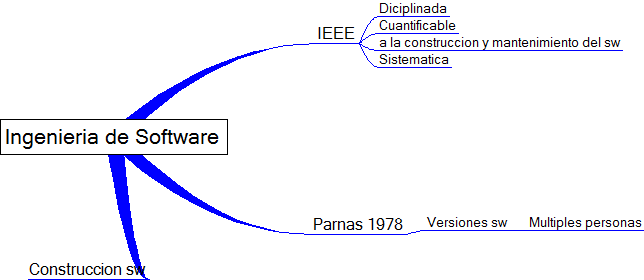
\includegraphics[angle=0,width=80mm]{capitulo1/definiciones_cppa.png} 
\caption{Definici\'on de Ingenier\'ia de software}
\label{figuragoogle}
\end{figure}

%Inlcuya el mapa mental de la definicion de IS
\begin{figure}[h!] \centering
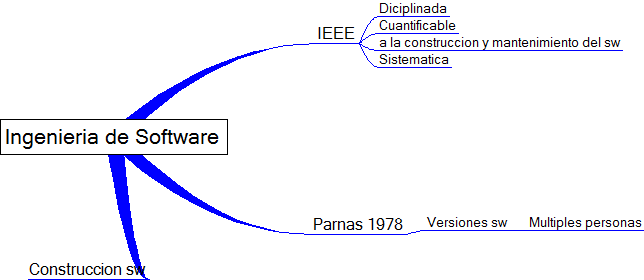
\includegraphics[angle=0,width=80mm]{capitulo1/definiciones_cppa.png} 
\caption{Definici\'on de Ingenier\'ia de software}
\label{figuragoogle}
\end{figure}


\chapter{Cualidades del software}

\subsection*{2.1 Discuta el impacto de las interfaces de usuarios sobre confiable}

\textbf{Claudia Patricia Prieto:}
\begin{quote}
Si los errores del software no son muy grandes aun asi es confiable.
\end{quote}

\textbf{Ramiro Hinostroza Rodriguez:}
\begin{quote}
Los clientes se esperan desde un principio que las primeras versiones de un software contengan errores.
\end{quote}

\textbf{José Manuel de Jesús Rodríguez Sotelo:}
\begin{quote}
Normalmente se avisa de la cantidad de errores que se han encontrado en el producto de software, pero esto no quiere decir que el producto pueda ser lanzado sin preocupación alguna, ya que no construyes un puente con una advertencia de "no usar".
\end{quote}

\textbf{Nancy Mayela Silva Martinez:}
\begin{quote}
Un sistema de software el cual es presentado al usuario promedio mediante una interfaz de ventana resulta más amigable que uno el cual requiera que el usuario ingrese varios conjuntos de comandos, causando que se dedique mas tiempo al desarrollo de la interfaz que al sistema en si.
\end{quote}

\textbf{Raul Bañuelos Hernandez:}
\begin{quote}
Muchos también utilizamos los términos corrección, robustez y fiabilidad en relación con el proceso de producción del software.
\end{quote}
%\input{capitulo3/cap3_3.1_3.2_3.3_Aldo_Haro}

%\begin{figure}[h!]\centring

\end{document}
